% Brent法のアルゴリズム図示と収束過程
\subsection{アルゴリズムの図示}
  \begin{figure}[H]
    \centering
    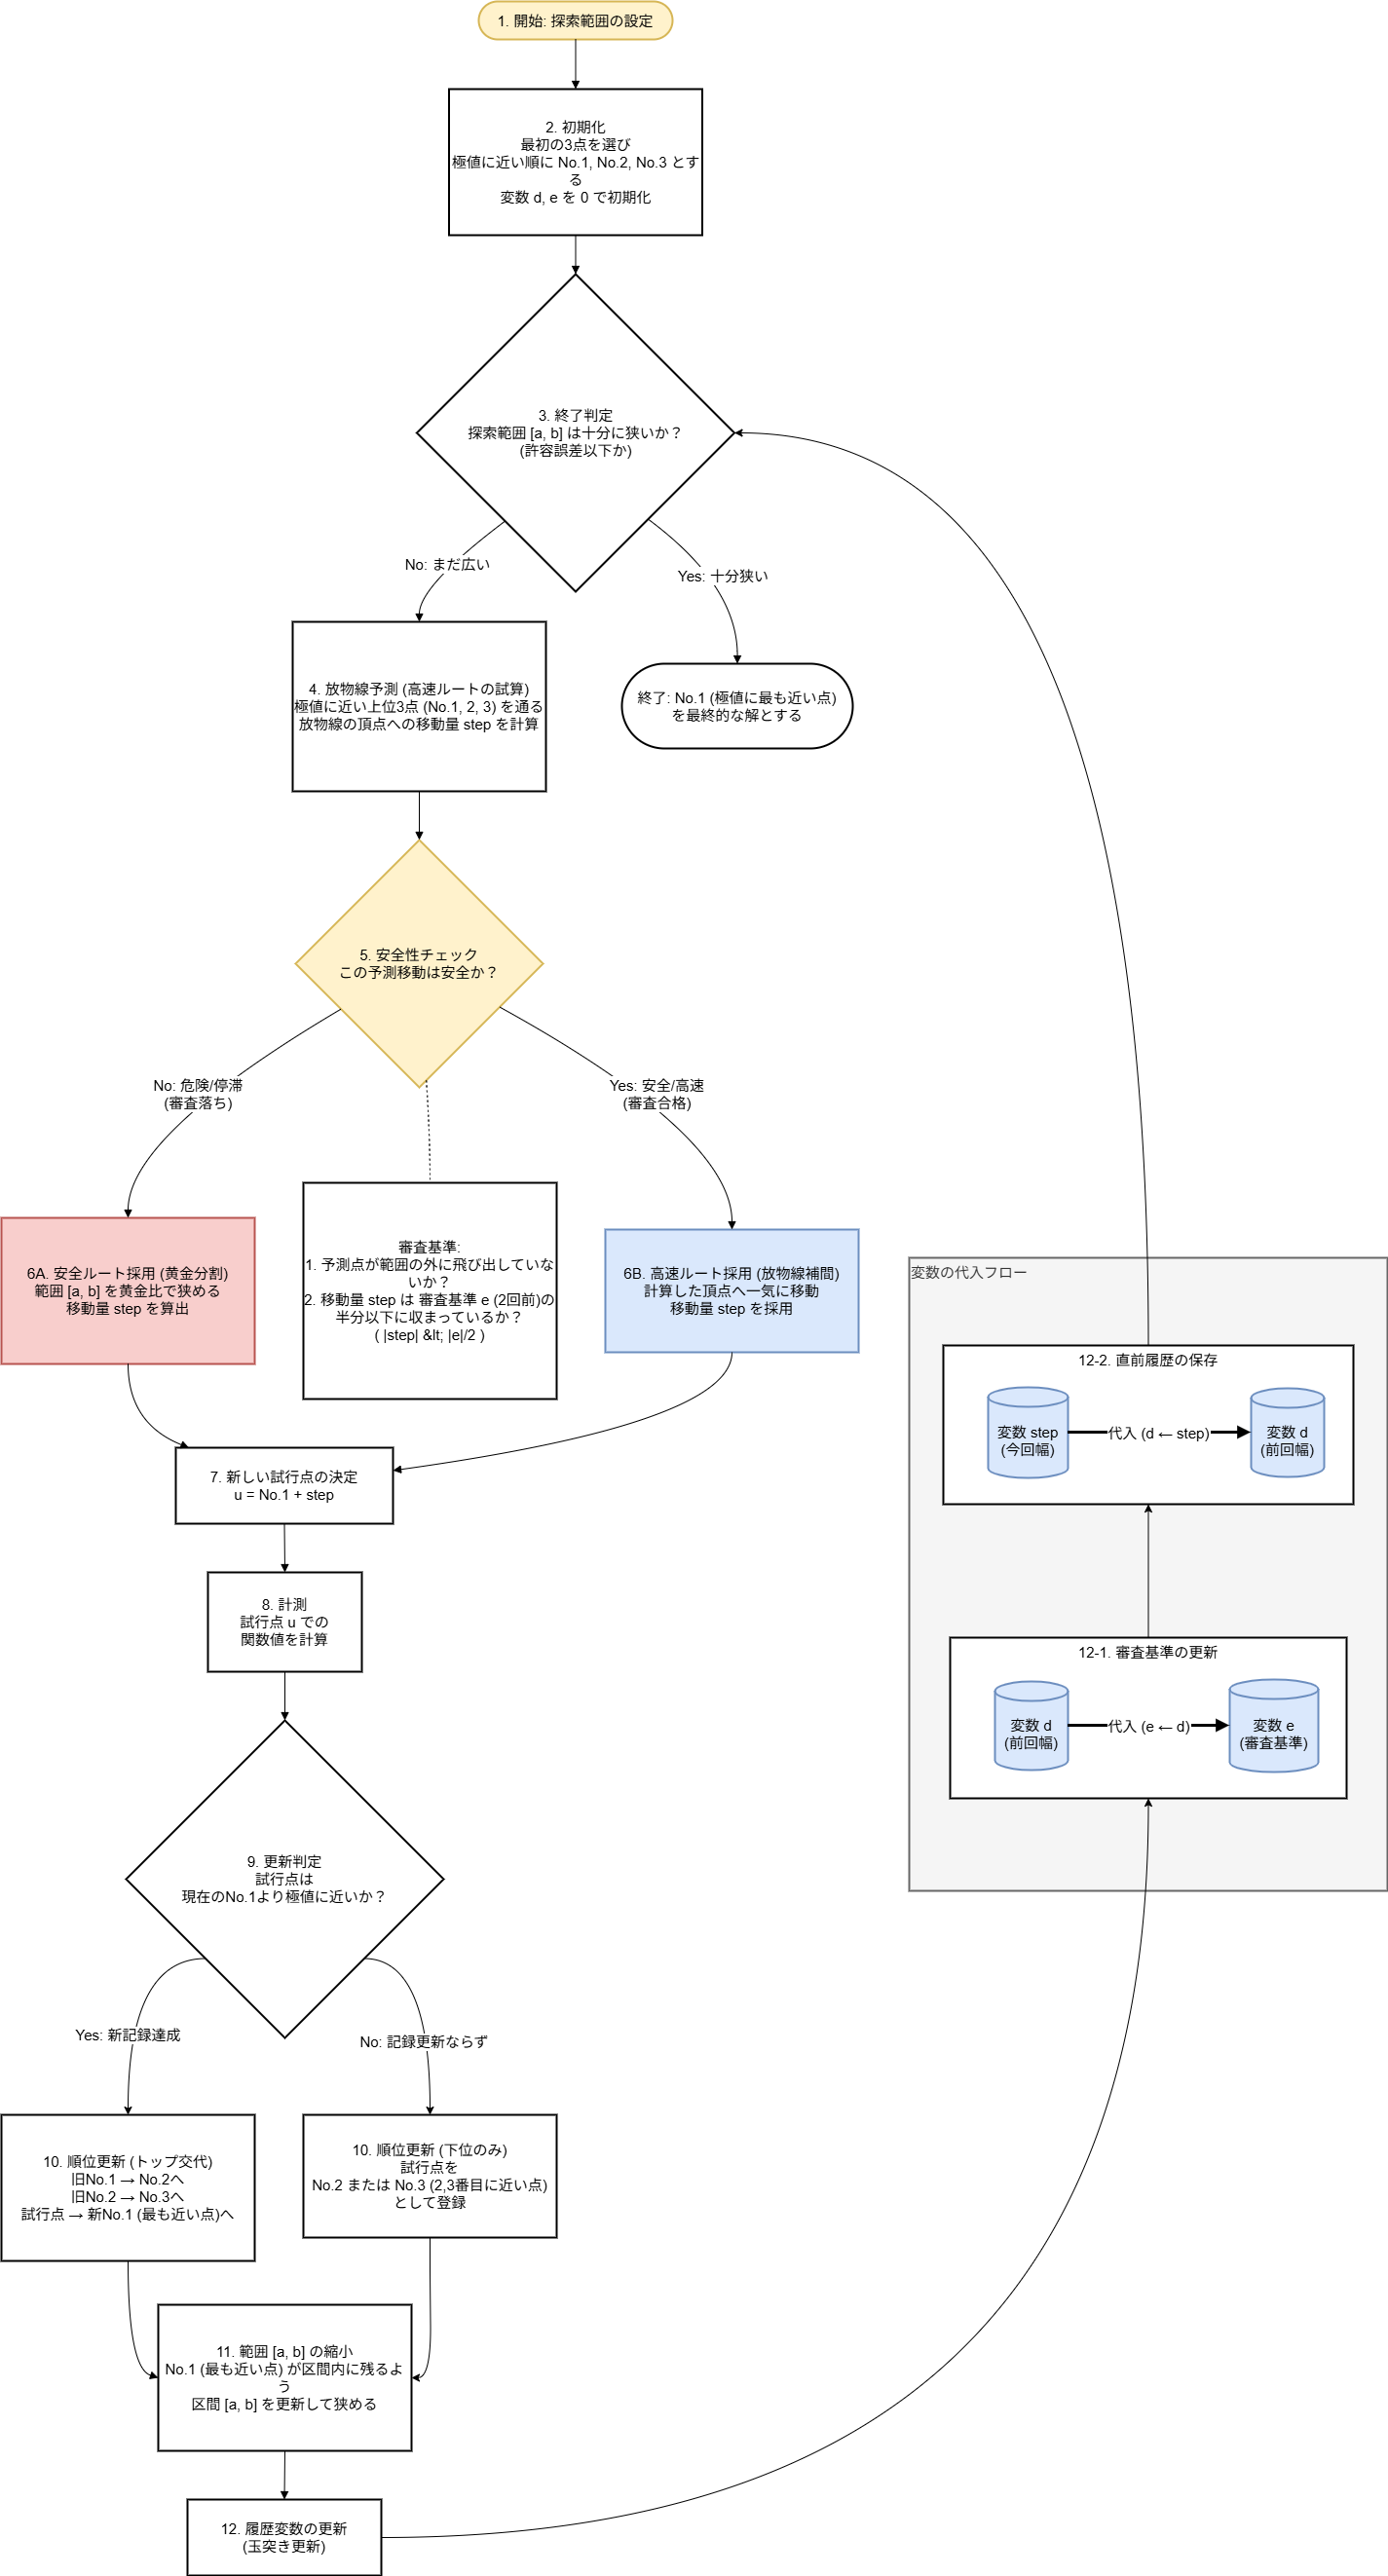
\includegraphics[width=0.7\linewidth]{material/brent/brent-architecture.png}
    \caption{Brent法のアルゴリズム構成}
  \end{figure}

\subsection{収束の様子}
  \begin{figure}[H]
    \begin{minipage}[b]{0.48\linewidth}
      \centering
      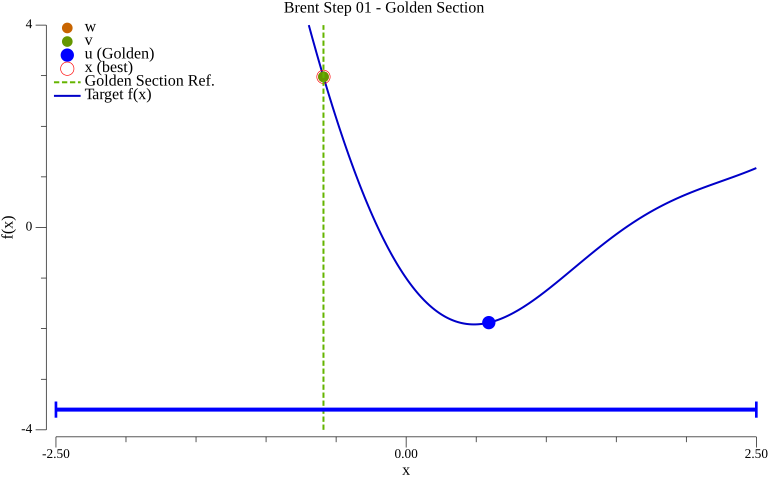
\includegraphics[width=1.0\linewidth]{material/brent/brent-step-01.png}
      \caption{Brent法-01回目}
    \end{minipage}
    \hfill
    \begin{minipage}[b]{0.48\linewidth}
      \centering
      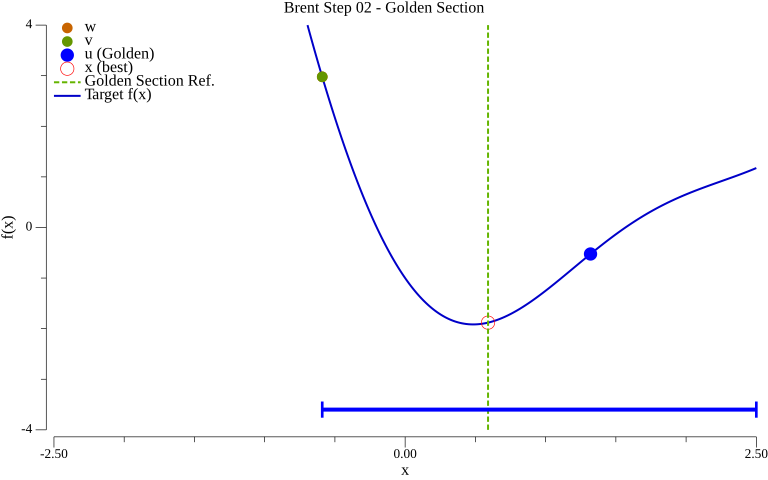
\includegraphics[width=1.0\linewidth]{material/brent/brent-step-02.png}
      \caption{Brent法-02回目}
    \end{minipage}
  \end{figure}
  \begin{figure}[H]
    \begin{minipage}[b]{0.48\linewidth}
      \centering
      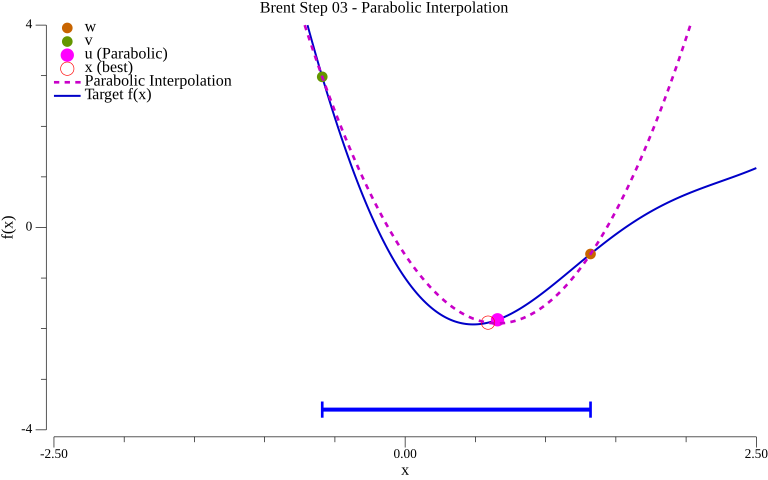
\includegraphics[width=1.0\linewidth]{material/brent/brent-step-03.png}
      \caption{Brent法-03回目}
    \end{minipage}
    \hfill
    \begin{minipage}[b]{0.48\linewidth}
      \centering
      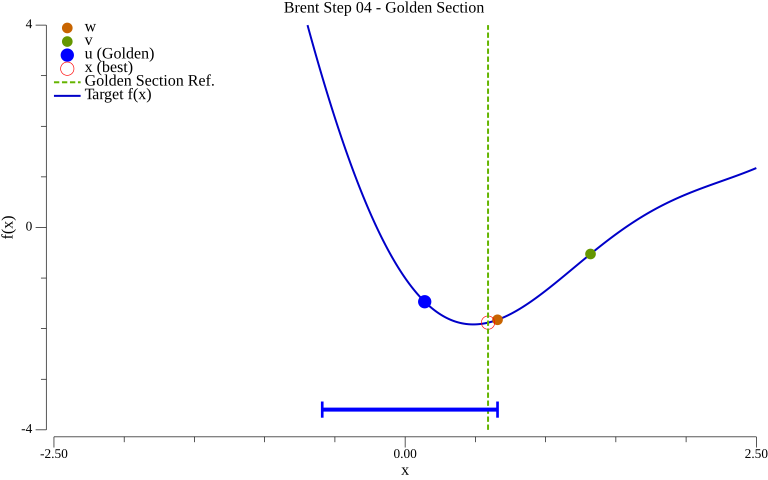
\includegraphics[width=1.0\linewidth]{material/brent/brent-step-04.png}
      \caption{Brent法-04回目}
    \end{minipage}
  \end{figure}
  \begin{figure}[H]
    \begin{minipage}[b]{0.48\linewidth}
      \centering
      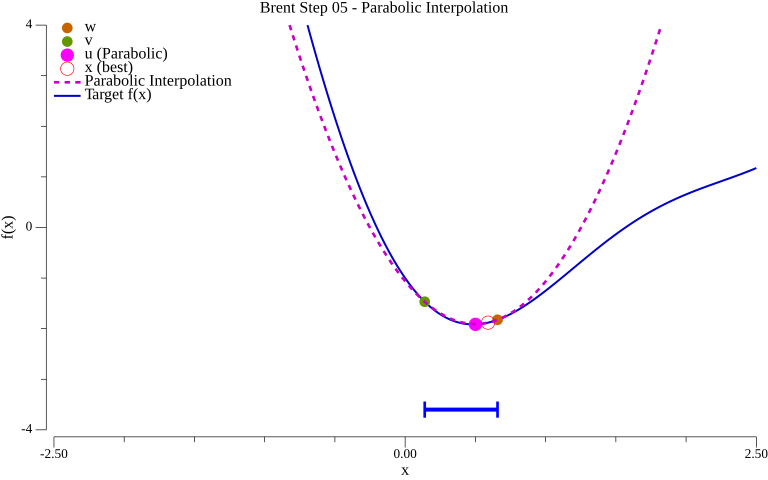
\includegraphics[width=1.0\linewidth]{material/brent/brent-step-05.png}
      \caption{Brent法-05回目}
    \end{minipage}
    \hfill
    \begin{minipage}[b]{0.48\linewidth}
      \centering
      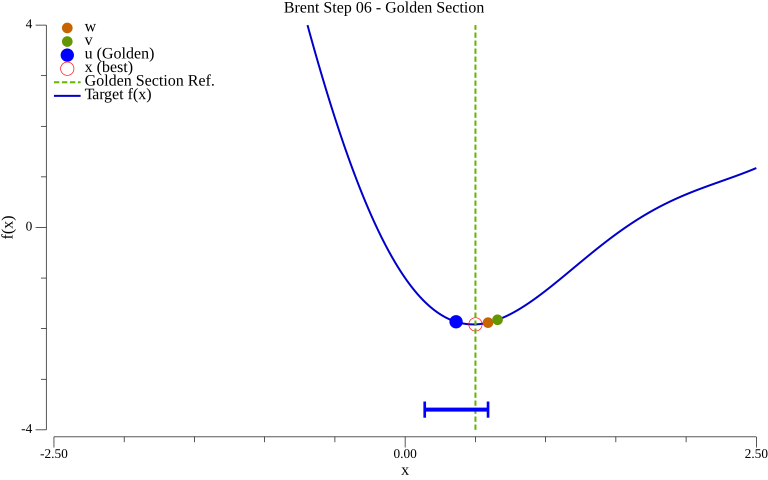
\includegraphics[width=1.0\linewidth]{material/brent/brent-step-06.png}
      \caption{Brent法-06回目}
    \end{minipage}
  \end{figure}
  \begin{figure}[H]
    \begin{minipage}[b]{0.48\linewidth}
      \centering
      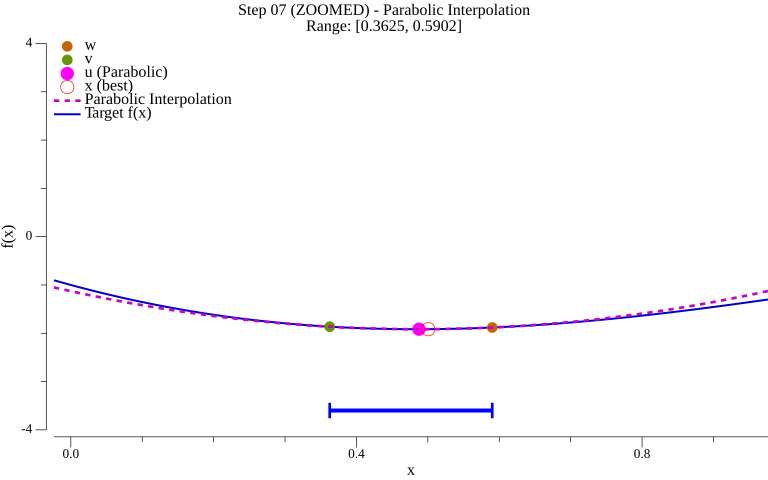
\includegraphics[width=1.0\linewidth]{material/brent/brent-step-07.png}
      \caption{Brent法-07回目}
    \end{minipage}
    \hfill
    \begin{minipage}[b]{0.48\linewidth}
      \centering
      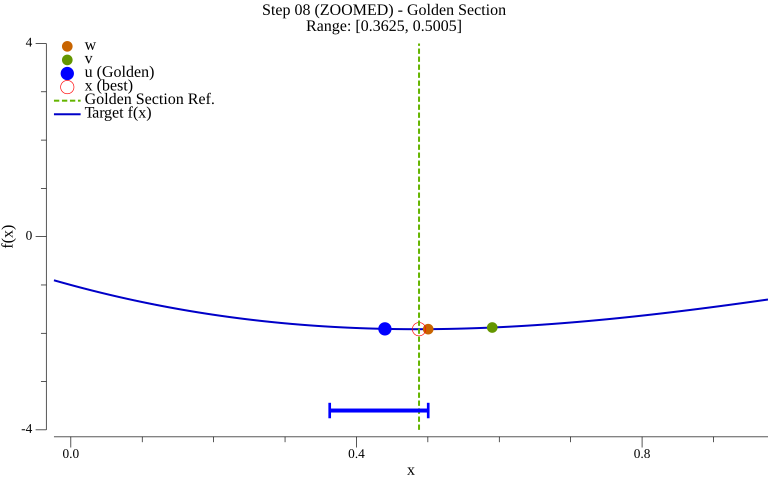
\includegraphics[width=1.0\linewidth]{material/brent/brent-step-08.png}
      \caption{Brent法-08回目}
    \end{minipage}
  \end{figure}
  \begin{figure}[H]
    \begin{minipage}[b]{0.48\linewidth}
      \centering
      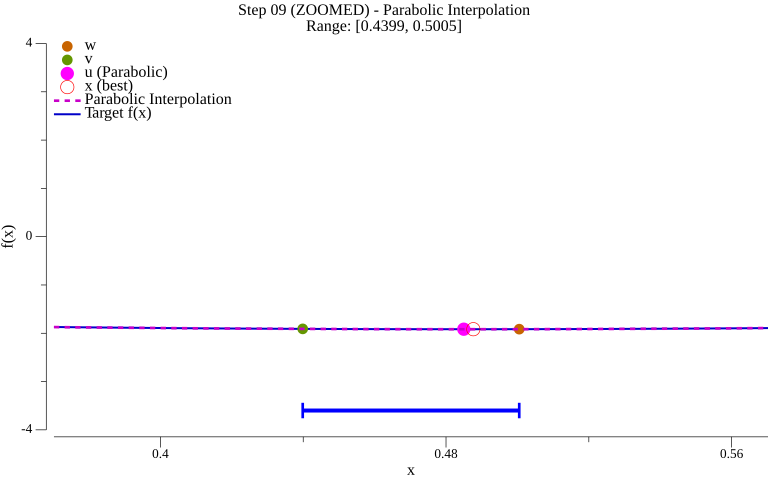
\includegraphics[width=1.0\linewidth]{material/brent/brent-step-09.png}
      \caption{Brent法-09回目}
    \end{minipage}
    \hfill
    \begin{minipage}[b]{0.48\linewidth}
      \centering
      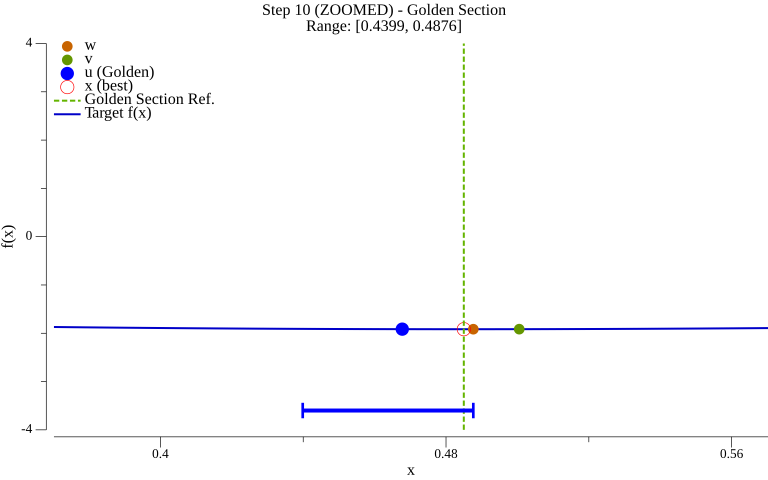
\includegraphics[width=1.0\linewidth]{material/brent/brent-step-10.png}
      \caption{Brent法-10回目}
    \end{minipage}
  \end{figure}
  \begin{figure}[H]
    \begin{minipage}[b]{0.48\linewidth}
      \centering
      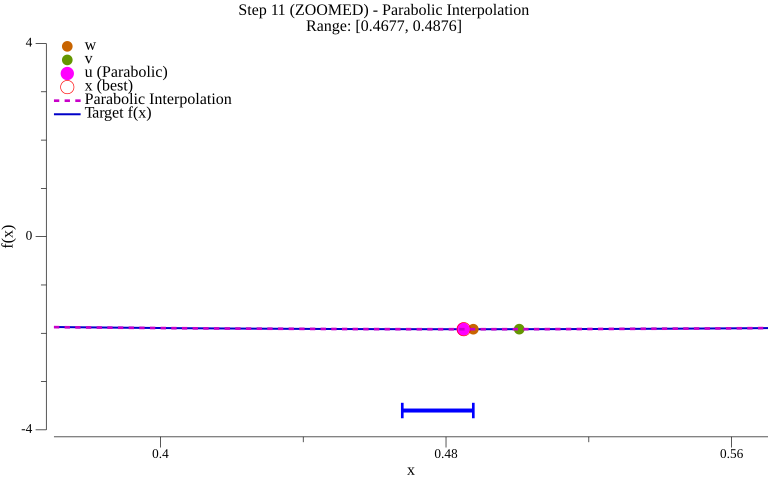
\includegraphics[width=1.0\linewidth]{material/brent/brent-step-11.png}
      \caption{Brent法-11回目}
    \end{minipage}
    \hfill
    \begin{minipage}[b]{0.48\linewidth}
      \centering
      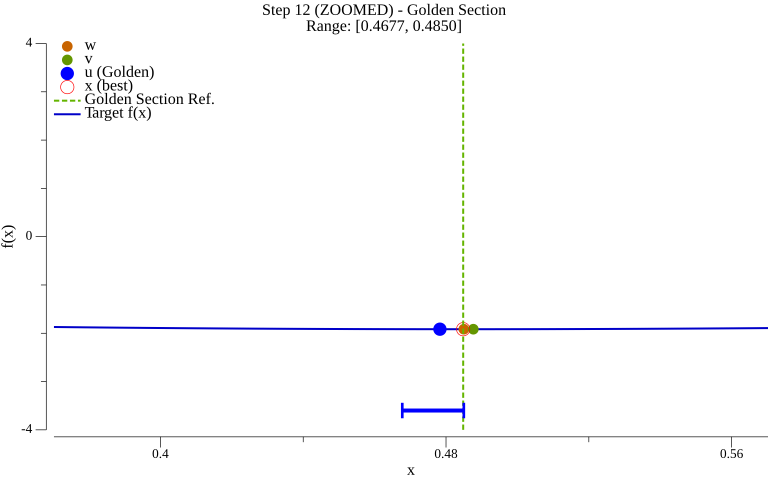
\includegraphics[width=1.0\linewidth]{material/brent/brent-step-12.png}
      \caption{Brent法-12回目}
    \end{minipage}
  \end{figure}
  \begin{figure}[H]
    \begin{minipage}[b]{0.48\linewidth}
      \centering
      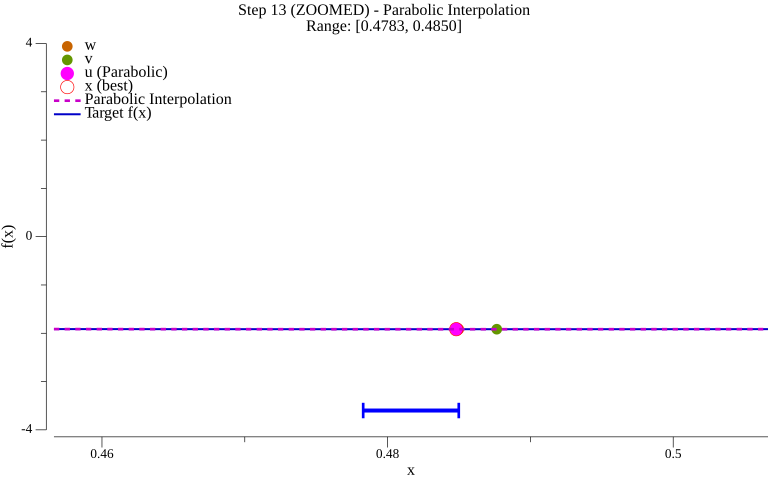
\includegraphics[width=1.0\linewidth]{material/brent/brent-step-13.png}
      \caption{Brent法-13回目}
    \end{minipage}
    \hfill
    \begin{minipage}[b]{0.48\linewidth}
      \centering
      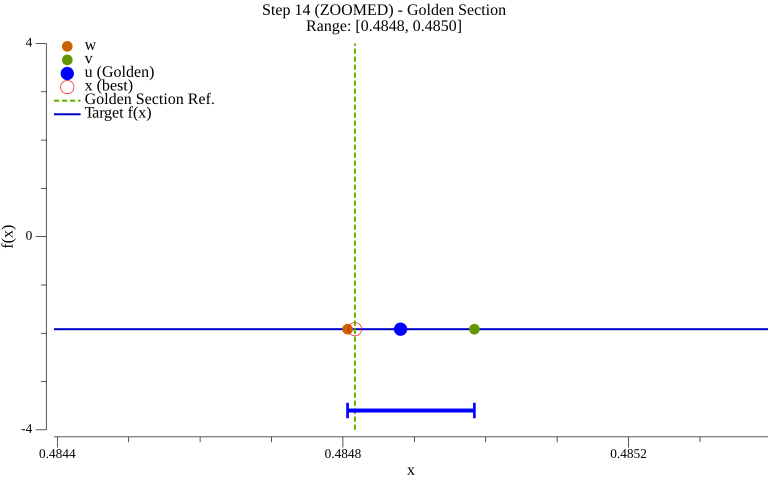
\includegraphics[width=1.0\linewidth]{material/brent/brent-step-14.png}
      \caption{Brent法-14回目}
    \end{minipage}
  \end{figure}
  \begin{figure}[H]
    \begin{minipage}[b]{0.48\linewidth}
      \centering
      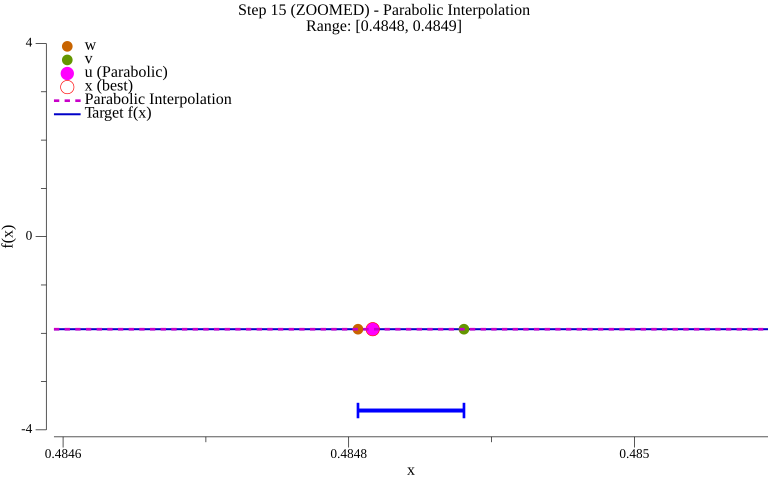
\includegraphics[width=1.0\linewidth]{material/brent/brent-step-15.png}
      \caption{Brent法-15回目}
    \end{minipage}
    \hfill
    \begin{minipage}[b]{0.48\linewidth}
      \centering
      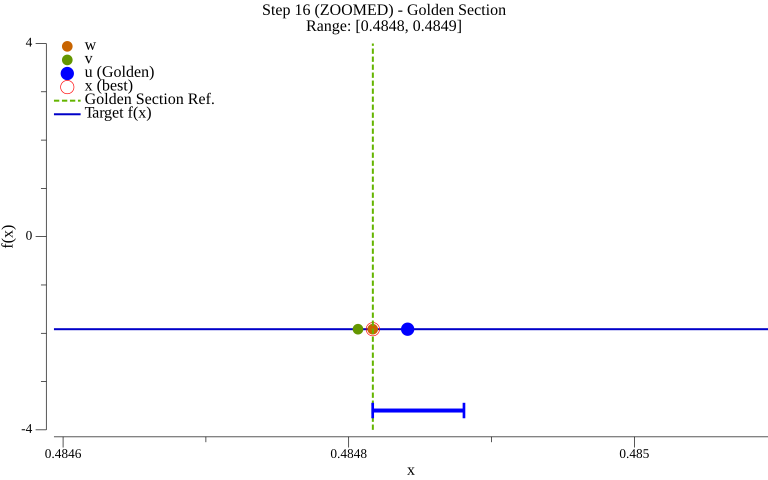
\includegraphics[width=1.0\linewidth]{material/brent/brent-step-16.png}
      \caption{Brent法-16回目}
    \end{minipage}
  \end{figure}
  \begin{figure}[H]
    \begin{minipage}[b]{0.48\linewidth}
      \centering
      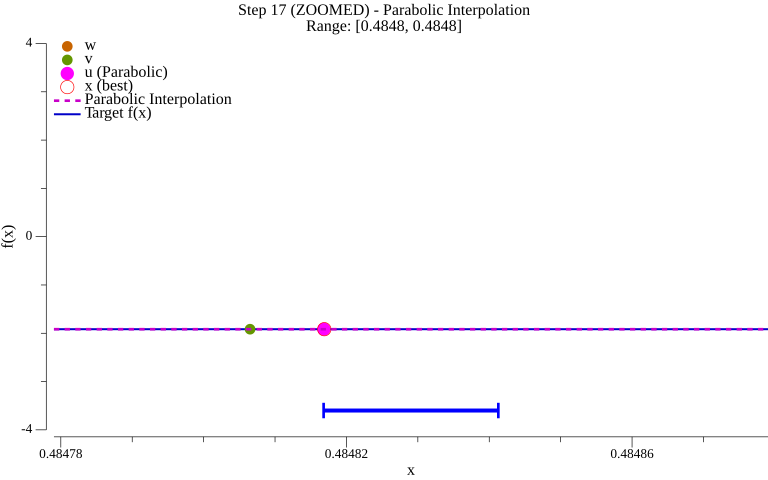
\includegraphics[width=1.0\linewidth]{material/brent/brent-step-17.png}
      \caption{Brent法-17回目}
    \end{minipage}
    \hfill
    \begin{minipage}[b]{0.48\linewidth}
      \centering
      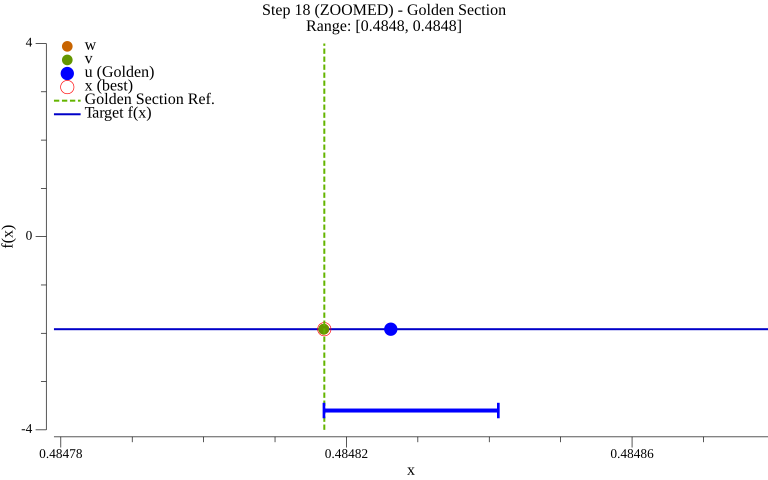
\includegraphics[width=1.0\linewidth]{material/brent/brent-step-18.png}
      \caption{Brent法-18回目}
    \end{minipage}
  \end{figure}
  \begin{figure}[H]
    \begin{minipage}[b]{0.48\linewidth}
      \centering
      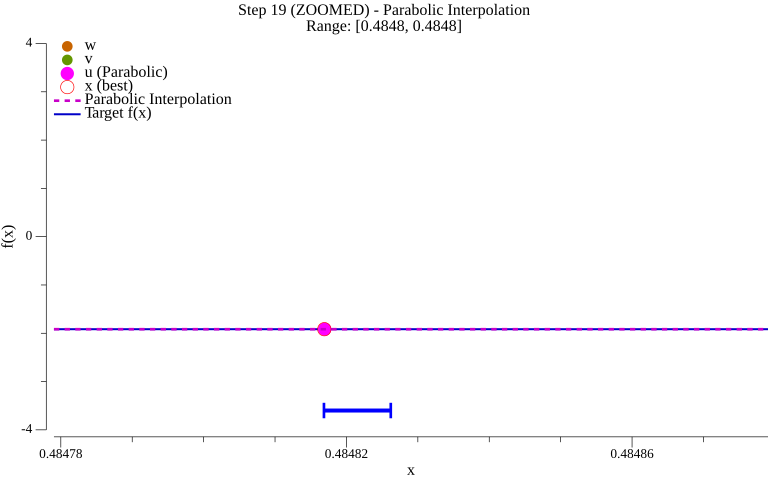
\includegraphics[width=1.0\linewidth]{material/brent/brent-step-19.png}
      \caption{Brent法-19回目}
    \end{minipage}
  \end{figure}
  \begin{figure}[H]
    \centering
    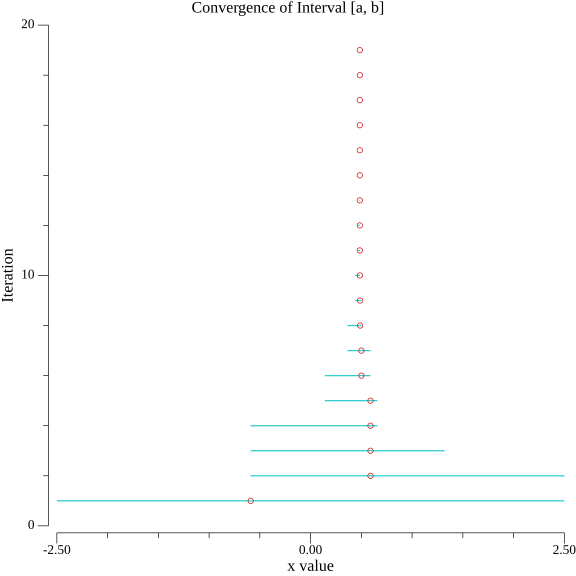
\includegraphics[width=0.7\linewidth]{material/brent/brent-interval.png}
    \caption{Brent法: 探索区間の収束推移}
  \end{figure}
